%%%%%%%%%%%%%%%%%%%%%%%%%%%%%%%%%%%%%%%%%
% Beamer Presentation
% LaTeX Template
% Version 1.0 (10/11/12)
%
% This template has been downloaded from:
% http://www.LaTeXTemplates.com
%
% License:
% CC BY-NC-SA 3.0 (http://creativecommons.org/licenses/by-nc-sa/3.0/)
%
%%%%%%%%%%%%%%%%%%%%%%%%%%%%%%%%%%%%%%%%%

%------------------------------------------------------------------------------------------------
% PACKAGES AND THEMES
%------------------------------------------------------------------------------------------------

\documentclass[table, xcolor = {dvipsnames}, 9pt]{beamer}
\usepackage{tikz}
\usetikzlibrary{calc}
\usetikzlibrary{positioning}
\usetikzlibrary{arrows.meta}
\usetikzlibrary{external}
\mode<presentation> {

% The Beamer class comes with a number of default slide themes
% which change the colors and layouts of slides. Below this is a list
% of all the themes, uncomment each in turn to see what they look like.

\usetheme{default}
%\usetheme{AnnArbor}
%\usetheme{Antibes}
%\usetheme{Bergen}
%\usetheme{Berkeley}
%\usetheme{Berlin}
%\usetheme{Boadilla}
%\usetheme{CambridgeUS}
%\usetheme{Copenhagen}
%\usetheme{Darmstadt}
%\usetheme{Dresden}
%\usetheme{Frankfurt}
%\usetheme{Goettingen}
%\usetheme{Hannover}
%\usetheme{Ilmenau}
%\usetheme{JuanLesPins}
%\usetheme{Luebeck}
%\usetheme{Madrid}
\usetheme{metropolis}
%\usetheme{Malmoe}
%\usetheme{Marburg}
%\usetheme{Montpellier}
%\usetheme{PaloAlto}
%\usetheme{Pittsburgh}
%\usetheme{Rochester}
%\usetheme{Singapore}
%\usetheme{Szeged}
%\usetheme{Warsaw}

% As well as themes, the Beamer class has a number of color themes
% for any slide theme. Uncomment each of these in turn to see how it
% changes the colors of your current slide theme.

%\usecolortheme{albatross}
%\usecolortheme{beaver}
%\usecolortheme{beetle}
%\usecolortheme{crane}
%\usecolortheme{dolphin}
%\usecolortheme{dove}
%\usecolortheme{fly}
%\usecolortheme{lily}
%\usecolortheme{orchid}
%\usecolortheme{rose}
\usecolortheme{seagull}
%\usecolortheme{seahorse}
%\usecolortheme{whale}
%\usecolortheme{wolverine}
\usefonttheme{professionalfonts}
%\setbeamertemplate{footline} % To remove the footer line in all slides uncomment this line
%\setbeamertemplate{footline}[page number] % To replace the footer line in all slides with a simple slide count uncomment this line

%\setbeamertemplate{navigation symbols}{} % To remove the navigation symbols from the bottom of all slides uncomment this line
}

\usepackage{graphicx} % Allows including images
\usepackage{booktabs} % Allows the use of \toprule, \midrule and \bottomrule in tables
\usepackage{tikz}
\usepackage{multirow}
\usepackage{natbib}
\usepackage{hyperref}
\usepackage{diagbox}
\usepackage{makecell}
\usepackage{xparse}
\usepackage{subfig}
\usepackage{amsmath}
\usepackage{amsfonts,amsthm,amsmath,amssymb}    
\usepackage{bbm}
\usepackage{bm}
\usepackage{empheq}
\usepackage{pgfplots}
\usepackage{animate}
\usepgfplotslibrary{colorbrewer}
\pgfplotsset{compat=1.17}

\newcommand\mybox[2][]{\tikz[overlay]\node[fill=lightgray,inner sep=2pt, anchor=text, rectangle, rounded corners=1mm,#1] {#2};\phantom{#2}}
\hypersetup{unicode=true,
            bookmarksnumbered=true,
            bookmarksopen=true,
            bookmarksopenlevel=2,
            breaklinks=false,
            pdfborder={0 0 1},
            hypertexnames=false,
            pdfstartview={XYZ null null 1}}
\usepackage{xcolor}
% R code listing style (matches the course's R-code slides)
\usepackage{listings}
\definecolor{codegreen}{rgb}{0,0.6,0}
\definecolor{codegray}{rgb}{0.5,0.5,0.5}
\definecolor{codepurple}{rgb}{0.58,0,0.82}
\definecolor{backcolour}{rgb}{0.95,0.95,0.92}
\lstdefinestyle{Rstyle}{
    language=R,
    backgroundcolor=\color{backcolour},
    commentstyle=\color{codegreen},
    keywordstyle=\color{magenta},
    stringstyle=\color{codepurple},
    basicstyle=\ttfamily\footnotesize,
    breakatwhitespace=false,
    breaklines=true,
    keepspaces=true,
    showspaces=false,
    showstringspaces=false,
    showtabs=false,
    tabsize=2
}
\newcommand\myheading[1]{%
  \par\bigskip
  {\Large\bfseries#1}\par\smallskip}
\newcommand\given[1][]{\:#1\vert\:}
\theoremstyle{plain}
\newtheorem{thm}{Theorem}
\newtheorem{prop}{Proposition\thisthmnumber}
\newtheorem{lem}{Lemma\thisthmnumber}
\newtheorem{cor}{Corollary}
\newtheorem{defin}{Definition}
\newtheorem{algo}{Algorithm}
\newcommand*\diff{\mathop{}\!\mathrm{d}}
\newcommand*\Diff[1]{\mathop{}\!\mathrm{d^#1}}
\newcommand{\bh}[1]{{\color{blue}{#1}}}
\newcommand{\mh}[1]{{\color{magenta}{#1}}}
\newcommand{\thisthmnumber}{}
\newcommand{\tikzmark}[1]{\tikz[baseline,remember picture] \coordinate (#1) {};}
\newcommand*{\QEDA}{\hfill\ensuremath{\blacksquare}}%
\newcommand*{\QEDB}{\hfill\ensuremath{\square}}%
\DeclareMathOperator{\E}{\rm{E}}
\DeclareMathOperator{\R}{\mathbb{R}}
\DeclareMathOperator{\N}{\mathbb{N}}
\DeclareMathOperator{\Var}{\rm{Var}}
\DeclareMathOperator{\Cov}{\rm{Cov}}
\DeclareMathOperator{\Supp}{\rm{Supp}}
\DeclareMathOperator{\e}{\rm{e}}
\DeclareMathOperator{\F}{\mathcal{F}}
\DeclareMathOperator{\Z}{\mathcal{Z}}
\DeclareMathOperator{\logit}{\rm{logit}}
\DeclareMathOperator{\indep}{{\perp\!\!\!\perp}}
\DeclareMathOperator{\rank}{rank}
\DeclareMathOperator*{\argmin}{arg\,min}
\DeclareMathOperator*{\argmax}{arg\,max}
%\DeclareMathOperator{\Pr}{\rm{Pr}}
%------------------------------------------------------------------------
% TITLE PAGE
%-----------------------------------------------------------------------
\pagestyle{empty}
\title[]{Random assignment, Fisher's exact test, and potential outcomes} % The short title appears at the bottom of every slide, the full title is only on the title page

\author{Thomas Leavitt} % Your name
\institute[]{} % Your institution for the title page
\date{June 15, 2026} % Date, can be changed to a custom date

\begin{document}

\begin{frame}
\titlepage % Print the title page as the first slide
\end{frame}

%\begin{frame}
%\frametitle{Overview} % Table of contents slide, comment this block out to remove it
%\tableofcontents % Throughout your presentation, if you choose to use \section{} and \subsection{} commands, these will automatically be printed on this slide as an overview of your presentation
%\end{frame}

%-------------------------------------------------------------------------------------
% PRESENTATION SLIDES
%-------------------------------------------------------------------------------------
\section{Where we are headed}
\begin{frame}[t]
\frametitle{Where we are headed}
\vfill
We begin with the randomized experiment, then relax its control step by step:
\vfill
\begin{enumerate} \vfill
\item[] \textcolor{magenta}{Part 1: The randomized experimental ideal} \vfill
\begin{itemize} \vfill
\item Introduction to potential outcomes and random assignment \vfill
\item Estimation and inference in fully controlled randomized experiments \vfill
\end{itemize} \vfill
\item[] \textcolor{magenta}{Part 2: Imperfectly controlled randomized experiments} \vfill
\begin{itemize} \vfill
\item Noncompliance: When subjects don't comply with experiment's treatment \vfill
\item Attrition: When subjects don't report their outcomes \vfill
\end{itemize} \vfill
\item[] \textcolor{magenta}{Part 3: Observational studies (when subjects self-select into treatment)} \vfill
\begin{itemize} \vfill
\item Matching and assessments of ``covariate balance'' \vfill
\item As interest allows: regression discontinuity, difference-in-differences, interrupted time series, synthetic control \vfill
\end{itemize} \vfill
\item[] \textcolor{magenta}{Part 4: Sensitivity analysis} \vfill
\begin{itemize} \vfill
\item How would inferences change should crucial assumptions be false? \vfill
\end{itemize} \vfill
\end{enumerate}
\vfill
\end{frame}
%-------------------------------------------------------------------------------------
\begin{frame}[t]
\frametitle{Where we are headed}
\vfill
\begin{itemize} \vfill
\item Part 1: conceptual, covering core statistics from a \mh{randomization- (design-) based} perspective \vfill
\begin{itemize} \vfill
\item[$\star$] Often the most challenging part \vfill
\end{itemize} \vfill
\item Parts 2 - 4 emphasize computation in \texttt{R} \vfill
\begin{itemize} \vfill
\item Especially \texttt{R}'s \texttt{optmatch} package \vfill
\end{itemize} \vfill
\end{itemize} \vfill
\vfill
\end{frame}
\section{Randomized experiments}
\begin{frame}{Randomized experiments and causal inference}
\vfill
\begin{itemize}
\item Experiments are conceptually and practically central to causal inference \vfill
\begin{itemize} \vfill
\item Specifically experiments featuring control groups and random assignment \vfill
\end{itemize} \vfill
\item Often a \mh{methodological ideal} \vfill
\item Stats 101 principles: Bias, variance, $p$-values, confidence levels, etc. \vfill
\begin{itemize} \vfill
\item But without data sampled from a superpopulation \vfill
\item[] or a probabilistic outcome-generating mechanism \vfill
\end{itemize} \vfill
\item Today: \emph{why} random assignment matters, via Fisher's ``Lady Tasting Tea'' \vfill
\end{itemize} \vfill
\end{frame}
%-------------------------------------------------------------------------------------
\begin{frame}{Fisher's ``Lady Tasting Tea'' \citep[][p.~13]{fisher1935a}}
\vfill
\begin{center}
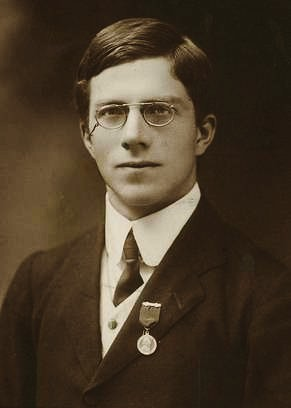
\includegraphics[height=0.8\textheight]{figures/RA_Fisher_1913.jpeg}%
\hspace{0.03\linewidth}%
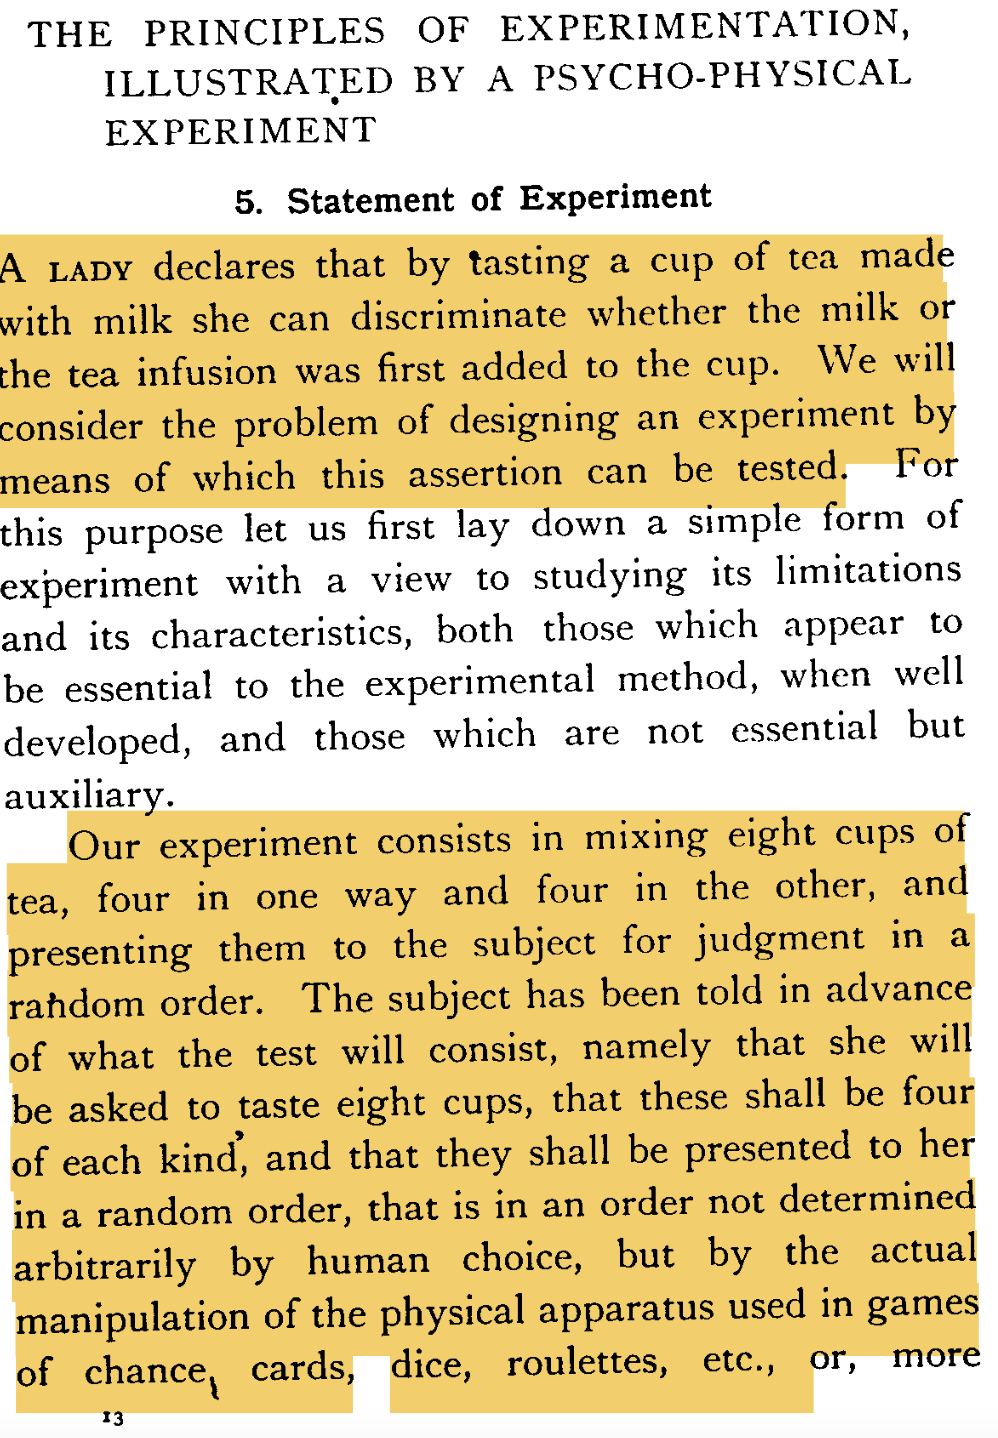
\includegraphics[height=0.8\textheight]{figures/Fisher_1935_P_13.png}
\end{center}
\vfill
\end{frame}
%-------------------------------------------------------------------------------------
\begin{frame}{Why randomize? The value of random assignment}
\vfill
\begin{itemize} \vfill
\item We see an apparent effect: is it \mh{real}, or just \mh{chance}? \vfill
\item Random assignment gives \mh{known, objective probabilities} \vfill
\begin{itemize} \vfill
\item fixed by the design, not by assumption \vfill
\end{itemize} \vfill
\item So the chance of a \mh{wrong conclusion} is known \vfill
\begin{itemize} \vfill
\item and ideally can be made \mh{small} by design \vfill
\end{itemize} \vfill
\item Randomization's value: a \mh{reasoned basis for inference} \vfill
\end{itemize} \vfill
\end{frame}
%-------------------------------------------------------------------------------------
\begin{frame}[t]{The Lady Tasting Tea: the setup}
\vfill
\begin{itemize} \vfill
\item Taster: $N = 8$ cups of tea \vfill
\item Each cup is prepared one of two ways \vfill 
\begin{itemize} \vfill 
\item \mh{milk-first} (treatment) or \mh{tea-first} (control) \vfill
\end{itemize} \vfill 
\item Cups sit in fixed positions, indexed $i \in \{1, \ldots, 8\}$ \vfill
\begin{itemize} \vfill
\item The \textbf{unit} is a cup; its position never changes \vfill
\end{itemize} \vfill
\item Goal: a high score should be \mh{strong evidence} she can discriminate \vfill
\item For that, a high score must be \mh{unlikely by chance} if she cannot \vfill
\item[] $\implies$ \textbf{randomize}, so that chance is \mh{known} \vfill
\end{itemize} \vfill
\end{frame}
%-------------------------------------------------------------------------------------
%-------------------------------------------------------------------------------------


\section{Random assignment}
\begin{frame}[t]{Treatment as a random variable (one cup)}
\vfill
\begin{itemize} \vfill
\item \textbf{Treatment}: a \textcolor{magenta}{random variable} $Z_i$ for cup $i$ \vfill
\begin{itemize} \vfill
\item ``We can think of a random variable as a container \ldots for a quantity that has yet to be determined by a random generative process'' \citep[][p.~16]{aronowmiller2019} \vfill
\end{itemize} \vfill
\item \textbf{Before} we prepare cup $i$, its treatment is \mh{unsettled} \vfill
\item[] so we write it as the uppercase random variable $Z_i$:
\begin{align*}
Z_i & =
\begin{cases}
1 & \text{if cup } i \text{ is milk-first (treatment)} \\
0 & \text{if cup } i \text{ is tea-first (control),}
\end{cases}
\end{align*}
with $Z_i = 1$ occurring with probability $\Pr\left(Z_i = 1\right)$ \vfill
\item \textbf{After} we prepare cup $i$, its treatment is \mh{settled} \vfill
\item[] so we write it as the lowercase value $z_i$: $z_i = 1$ or $z_i = 0$ \vfill
\end{itemize}
\vfill
\end{frame}
%-------------------------------------------------------------------------------------
\begin{frame}{The assignment vector $\bm{z}$}
\vfill
\begin{itemize} \vfill
\item \mh{Treatment assignment}: is cup $i$ milk-first ($z_i = 1$) or tea-first ($z_i = 0$)? \vfill
\item Collect all $N$ indicators in $\bm{z} = \begin{bmatrix} z_1 & z_2 & \ldots & z_N \end{bmatrix}^{\top}$ \vfill
\item $2^N$ ways to assign $N$ units to treatment or control \vfill
\end{itemize} \vfill
\begin{equation*}
\left\{0, 1\right\}^N = \left\{
\begin{bmatrix} 0 \\ 0 \\ 0 \\ 0 \\ 0 \\ 0 \\ 0 \\ 0 \end{bmatrix},
\begin{bmatrix} 1 \\ 0 \\ 0 \\ 0 \\ 0 \\ 0 \\ 0 \\ 0 \end{bmatrix},
\begin{bmatrix} 0 \\ 1 \\ 0 \\ 0 \\ 0 \\ 0 \\ 0 \\ 0 \end{bmatrix},
\cdots ,
\begin{bmatrix} 1 \\ 0 \\ 1 \\ 1 \\ 1 \\ 1 \\ 1 \\ 1 \end{bmatrix},
\begin{bmatrix} 0 \\ 1 \\ 1 \\ 1 \\ 1 \\ 1 \\ 1 \\ 1 \end{bmatrix},
\begin{bmatrix} 1 \\ 1 \\ 1 \\ 1 \\ 1 \\ 1 \\ 1 \\ 1 \end{bmatrix}
\right\}
\end{equation*} \vfill
\end{frame}
%---------------------------------------------------------------
\begin{frame}{A randomized design is a distribution over assignments}
\vfill
\begin{itemize} \vfill
\item A randomized design selects assignment from $\{0,1\}^N$ with probability $p(\bm{z})$ \vfill
\item So $\bm{Z}$ is a random vector, support $\Omega \coloneqq \left\{\bm{z}: p(\bm{z}) > 0\right\}$, $\Pr(\bm{Z} = \bm{z}) = p(\bm{z})$ \vfill
\item \mh{Bernoulli (simple) assignment}: $N$ independent (usually fair) coin flips \vfill
\item \mh{Complete random assignment}: draw $n_1$ ``treated'' balls from an urn of $N$ \vfill
\item The design ($\Omega$ and $p(\bm{z})$) is the one thing the researcher \emph{knows} \vfill
\end{itemize} \vfill
\end{frame}
%---------------------------------------------------------------
\begin{frame}{Fisher's design: four cups each way, random order}
\vfill
\begin{itemize} \vfill
\item \citet[][p.~13]{fisher1935a}: ``\ldots mixing eight cups of tea, four in one way and four in the other \ldots\ in a random order'' \vfill
\item Complete random assignment with $N = 8$, $n_1 = 4$ \vfill 
\item[] Support: $\binom{8}{4} = 70$ assignments \vfill
\begin{equation*}
\Omega = \left\{
\begin{bmatrix} 1 \\ 1 \\ 1 \\ 1 \\ 0 \\ 0 \\ 0 \\ 0 \end{bmatrix},
\begin{bmatrix} 1 \\ 1 \\ 1 \\ 0 \\ 1 \\ 0 \\ 0 \\ 0 \end{bmatrix},
\begin{bmatrix} 1 \\ 1 \\ 1 \\ 0 \\ 0 \\ 1 \\ 0 \\ 0 \end{bmatrix},
\cdots ,
\begin{bmatrix} 0 \\ 0 \\ 0 \\ 1 \\ 0 \\ 1 \\ 1 \\ 1 \end{bmatrix},
\begin{bmatrix} 0 \\ 0 \\ 0 \\ 0 \\ 1 \\ 1 \\ 1 \\ 1 \end{bmatrix}
\right\}
\end{equation*} \vfill
\item Each assignment is equally likely: $\Pr(\bm{Z} = \bm{z}) = 1/\lvert \Omega \rvert = 1/70$ for $\bm{z} \in \Omega$ \vfill
\begin{itemize} \vfill
\item $\lvert \Omega \rvert$ = number of assignments in $\Omega$ (here $70$) \vfill
\end{itemize} \vfill
\end{itemize} \vfill
\end{frame}
%% ============================================================
%% PART 3 --- FISHER'S EXACT TEST, ON HIS OWN TERMS
%% ============================================================
\section{Fisher's exact test}

\begin{frame}{The observed experiment and its test statistic}
\vfill
\begin{itemize} \vfill
\item One of the $70$ assignments is drawn; the taster judges each cup \vfill
\end{itemize} \vfill
\begin{table}[H]
\centering
\small
\begin{tabular}{c|cc}
\toprule
Unit & $\bm{z}$ (assigned) & $\bm{y}$ (judged milk-first) \\
  \midrule
$1$ & $1$ & $1$ \\
$2$ & $1$ & $1$ \\
$3$ & $1$ & $1$ \\
$4$ & $1$ & $1$ \\
$5$ & $0$ & $0$ \\
$6$ & $0$ & $0$ \\
$7$ & $0$ & $0$ \\
$8$ & $0$ & $0$
\end{tabular}
\end{table}
\vspace{-0.5em}
\begin{itemize} \vfill
\item \mh{Test statistic} $t(\bm{z},\bm{y})$: a \mh{rule} applied to $\bm{z}$ and $\bm{y}$, giving one number \vfill
\begin{itemize} \vfill 
\item[] Read as ``apply rule $t$'' to the assignment and the outcomes \vfill
\end{itemize} \vfill 
\item Our rule counts milk-first cups judged milk-first: $t(\bm{z},\bm{y}) = \bm{z}^{\top}\bm{y} = \sum_{i} z_i y_i = 4$ \vfill
\item How surprising is $4$ if she \mh{cannot discriminate}? \vfill
\end{itemize} \vfill
\end{frame}
%---------------------------------------------------------------
\begin{frame}{Fisher's move: vary the assignment, hold the judgments fixed}
\vfill
\begin{itemize} \vfill
\item Under \mh{no discrimination}, each judgment is the same either way the cup was poured \vfill
\begin{itemize} \vfill
\item so hold the observed judgments $\bm{y}$ \mh{fixed} (no potential outcomes needed) \vfill
\end{itemize} \vfill
\item The experiment ran \mh{once}: only one assignment was realized \vfill
\item Fisher asks what $t$ \emph{would have been}: \vfill
\begin{itemize} \vfill
\item across the assignments the randomization \mh{could have produced} \vfill
\item the ``what if'' is in the \mh{assignment}, not the outcomes \vfill
\end{itemize} \vfill
\item Randomization makes the assignment probabilities $p(\bm{z})$ \mh{known} \vfill
\begin{itemize} \vfill
\item so the distribution of $t$ under no discrimination is \mh{known} \vfill
\item equal probabilities (here) make it especially simple \vfill
\end{itemize} \vfill
\end{itemize} \vfill
\end{frame}
%---------------------------------------------------------------
\begin{frame}{Reassigning labels under no discrimination (outcomes fixed)}
\vfill
\begin{itemize} \vfill
\item Hold $\bm{y}$ at its observed values; recompute $\bm{z}^{\top}\bm{y}$ as $\bm{z}$ sweeps $\Omega$ \vfill
\end{itemize} \vfill
\begin{table}[H]
\scriptsize
    \begin{tabular}{l|l}
    \toprule
    $\mathbf{z}_1$ & $\mathbf{y}$ \\ \midrule
    1 & 1  \\ 1 & 1 \\ 1 & 1 \\ 1 & 1 \\ 0 & 0 \\ 0 & 0 \\ 0 & 0 \\ 0 & 0
    \end{tabular}
    \hfill
      \begin{tabular}{l|l}
      \toprule
    $\mathbf{z}_2$ & $\mathbf{y}$ \\ \midrule
    1 & 1 \\ 1 & 1 \\ 1 & 1 \\ 0 & 1 \\ 1 & 0 \\ 0 & 0 \\ 0 & 0 \\ 0 & 0
    \end{tabular}
     \hfill
      \begin{tabular}{l|l}
      \toprule
    $\mathbf{z}_3$ & $\mathbf{y}$ \\ \midrule
    1 & 1 \\ 1 & 1 \\ 1 & 1 \\ 0 & 1 \\ 0 & 0 \\ 1 & 0 \\ 0 & 0 \\ 0 & 0
    \end{tabular}
     \hfill $\cdots$ \hfill
      \begin{tabular}{l|l}
      \toprule
    $\mathbf{z}_{69}$ & $\mathbf{y}$ \\ \midrule
    0 & 1 \\ 0 & 1 \\ 0 & 1 \\ 1 & 1 \\ 0 & 0 \\ 1 & 0 \\ 1 & 0 \\ 1 & 0
    \end{tabular}
     \hfill
      \begin{tabular}{l|l}
      \toprule
    $\mathbf{z}_{70}$ & $\mathbf{y}$ \\ \midrule
    0 & 1 \\ 0 & 1 \\ 0 & 1 \\ 0 & 1 \\ 1 & 0 \\ 1 & 0 \\ 1 & 0 \\ 1 & 0
    \end{tabular}
\end{table}
\vfill
\begin{itemize} \vfill
\item These $70$ values, equally likely here, form the \mh{randomization distribution} of $t$ under no discrimination \vfill
\end{itemize} \vfill
\end{frame}
%---------------------------------------------------------------
\begin{frame}{Is the observed result surprising?}
\vfill
\begin{center}
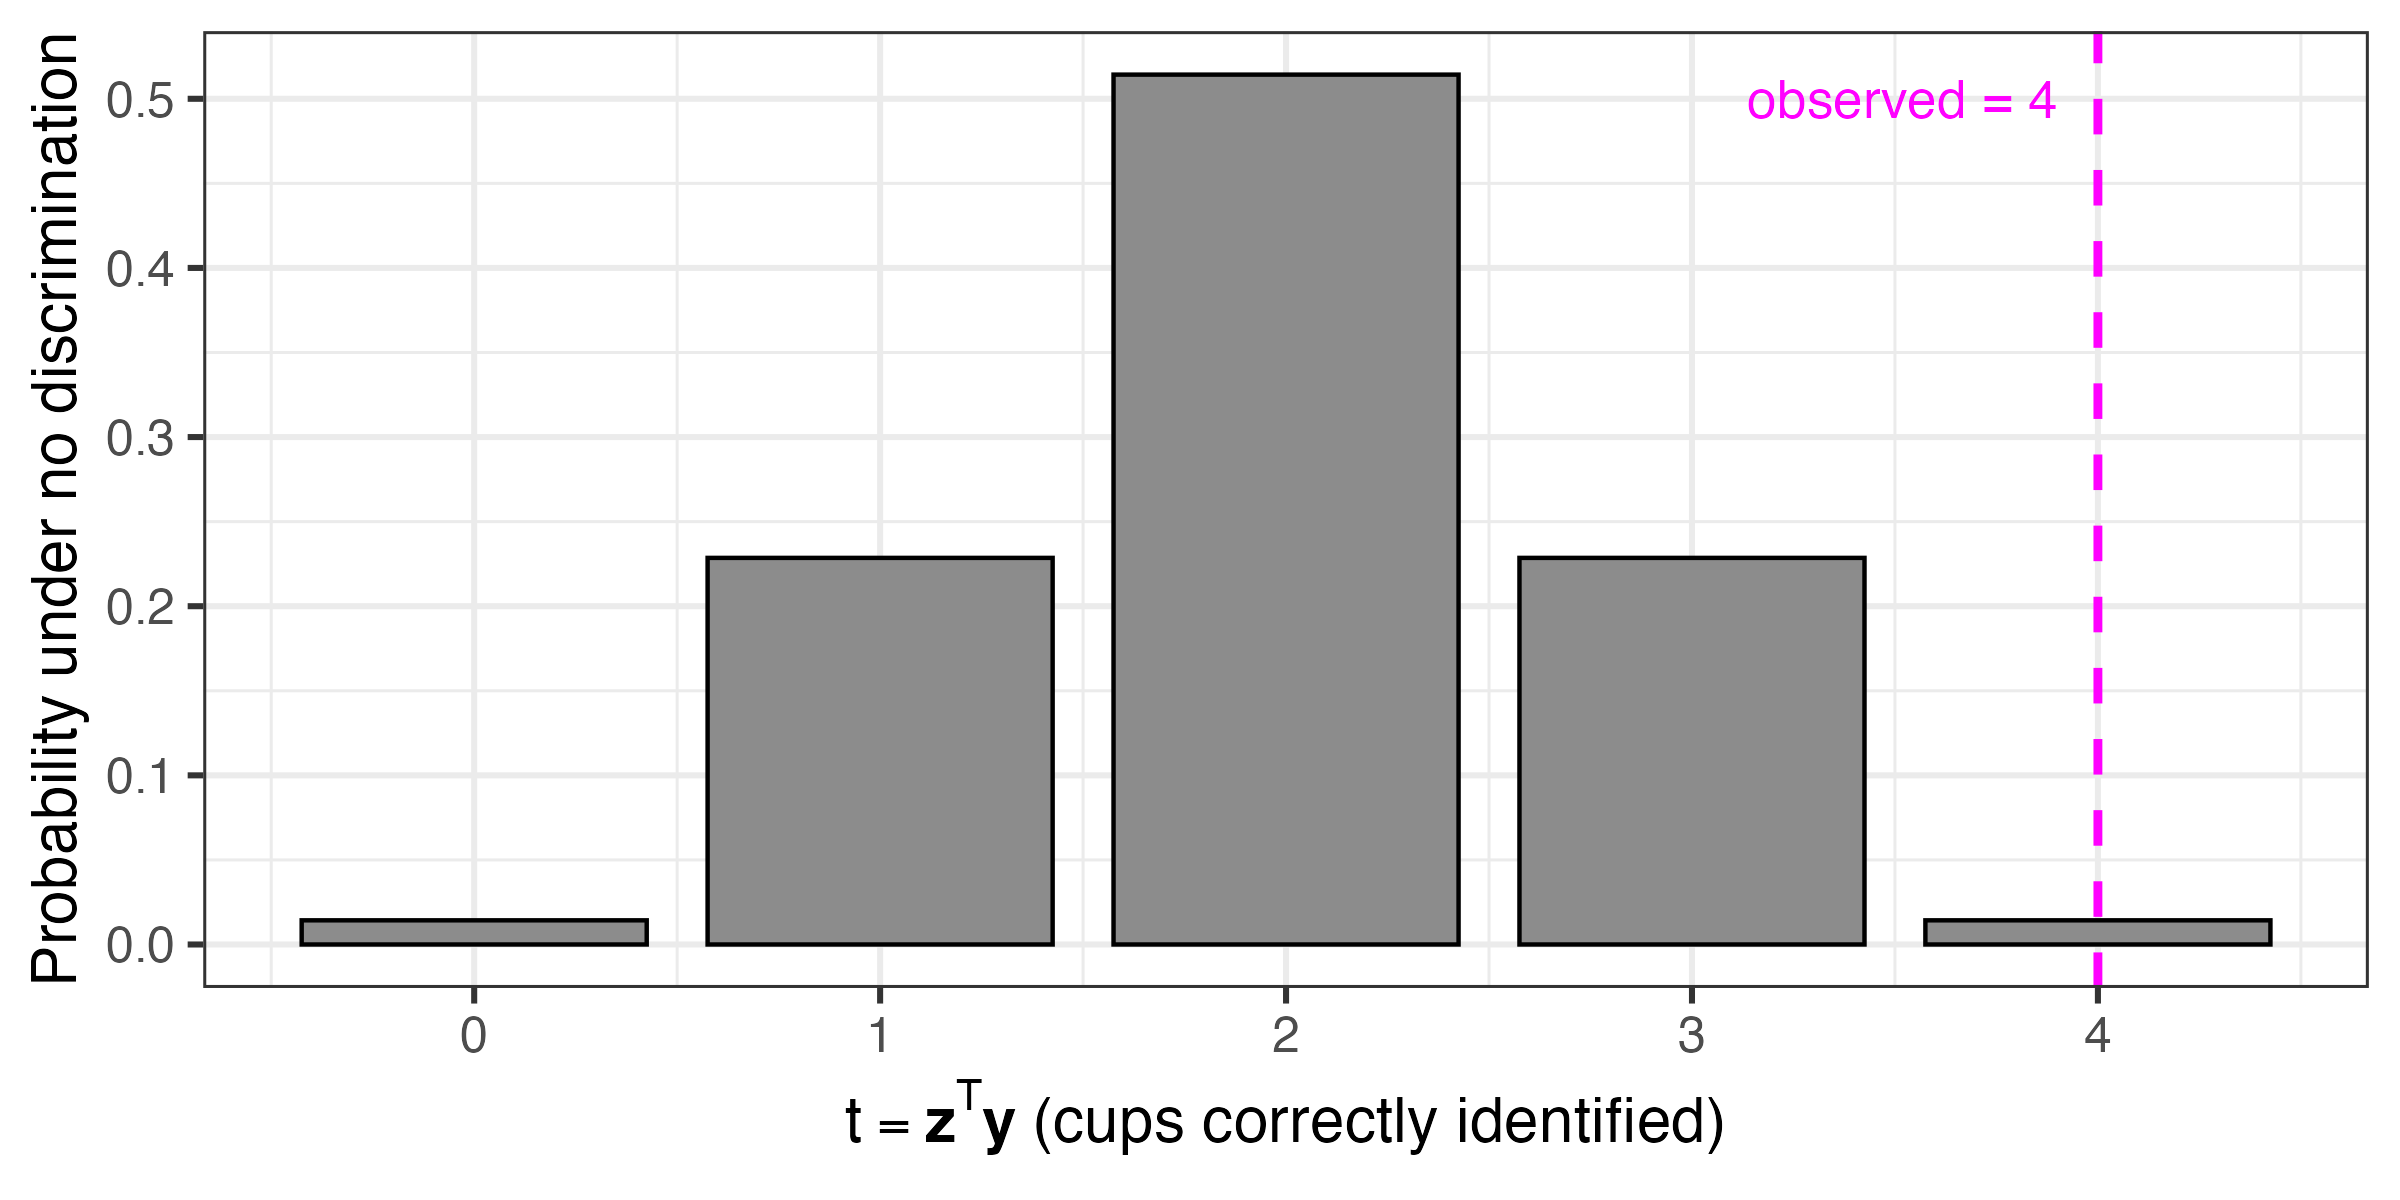
\includegraphics[height=0.52\textheight,keepaspectratio]{figures/fisher_null_dist.png}
\end{center}
\vspace{-0.5em}
\begin{itemize} \vfill
\item Only $1$ of $70$ assignments is this extreme: $\Pr(\bm{Z}^{\top}\bm{y} \geq 4) = 1/70 \approx 0.014$ \vfill
\item \mh{Rule}: reject no discrimination only when she gets all four correct \vfill
\begin{itemize} \vfill
\item wrongly reject only $1/70$ of the time when it is true \vfill
\end{itemize} \vfill
\end{itemize} \vfill
\end{frame}
%---------------------------------------------------------------
\begin{frame}[fragile]{Fisher's tea test in \texttt{R}}
\begin{lstlisting}[style=Rstyle, basicstyle=\ttfamily\tiny, frame=single]
# Observed assignment: 1 = milk-first, 0 = tea-first
z_obs <- c(1, 1, 1, 1, 0, 0, 0, 0)
# Taster's labels:     1 = says "milk-first", 0 = says "tea-first"
y_obs <- c(1, 1, 1, 1, 0, 0, 0, 0)

# Test statistic t = z^T y: number of milk-first cups (z = 1)
# that the taster also labels milk-first (y = 1)
t_obs <- sum(z_obs * y_obs)              # = 4 (all four correct)

# Every way to choose 4 of the 8 cups to be milk-first:
# choose(8, 4) = 70 possible assignments; the other 4 are tea-first
milk_first_sets <- combn(x = 1:8, m = 4)   # columns = the 70 choices

# Turn each choice of 4 cups into an assignment vector z
all_z <- apply(X = milk_first_sets, MARGIN = 2, FUN = function(cups) {
  z <- rep(x = 0, times = 8)             # start all tea-first
  z[cups] <- 1                           # set chosen cups milk-first
  z
})

# Recompute t = z^T y for each assignment, holding y_obs FIXED
all_t <- apply(X = all_z, MARGIN = 2, FUN = function(z) sum(z * y_obs))

# Under NO DISCRIMINATION (y fixed; z random by the known design),
# chance of a score as high as observed:
mean(all_t >= t_obs)                     # = 1/70 = 0.01428571
\end{lstlisting}
\end{frame}
%% ============================================================
%% PART 4 --- POTENTIAL OUTCOMES (THE MODERN LANGUAGE)
%% ============================================================
\section{Potential outcomes}

\begin{frame}{What did ``no discrimination'' assume?}
\vfill
\begin{itemize} \vfill
\item Strong evidence against \mh{no discrimination}: what did it claim about each cup? \vfill
\item That each cup's judgment is the \mh{same}, milk-first or tea-first \vfill
\item Name the two responses a cup could give: \vfill
\begin{itemize} \vfill
\item $y_i(1)$ if cup $i$ is milk-first, \quad $y_i(0)$ if cup $i$ is tea-first \vfill
\end{itemize} \vfill
\item These are \mh{potential outcomes} \citep{neyman1923,rubin1974} \vfill
\item No discrimination is exactly $y_i(1) = y_i(0)$ for every cup \vfill
\end{itemize} \vfill
\end{frame}
%---------------------------------------------------------------
\begin{frame}{A causal model specifies potential outcomes}
\vfill
\begin{itemize} \vfill
\item In general a cup's response could depend on the \emph{whole} assignment: $y_i(\bm{z})$ \vfill
\item A causal model specifies $y_i(\bm{z})$ for every $\bm{z} \in \{0,1\}^N$ \vfill
\item \mh{SUTVA} \citep{cox1958a,rubin1980b,rubin1986}: a cup responds only to its own $z_i$ \vfill
\begin{itemize} \vfill
\item no interference, and one version of each preparation \vfill
\end{itemize} \vfill
\item Under SUTVA the model gives two responses per cup: $y_i(1)$ and $y_i(0)$ \vfill
\end{itemize} \vfill
\end{frame}
%---------------------------------------------------------------
\begin{frame}{We observe only one response per cup}
\vfill
\begin{itemize} \vfill
\item We see one response per cup: $\; y_i = z_i\,y_i(1) + (1 - z_i)\,y_i(0)$ \vfill
\item The other response is never observed \vfill
\begin{itemize} \vfill
\item \mh{Fundamental Problem of Causal Inference} \citep{holland1986} \vfill
\end{itemize} \vfill
\item A \mh{sharp causal model} specifies both $y_i(1)$ and $y_i(0)$ for every cup \vfill
\item So we can compute $t(\bm{z},\bm{y})$ for any assignment, \\ and its randomization distribution \vfill
\item No discrimination, $y_i(1) = y_i(0)$, recovers Fisher's fixed responses \vfill
\end{itemize} \vfill
\end{frame}
%% ============================================================
%% PART 5 --- OTHER SHARP HYPOTHESES
%% ============================================================
\section{Other sharp models}

\begin{frame}{An alternative sharp model: perfect discrimination}
\vfill
\begin{itemize} \vfill
\item No discrimination is only \emph{one} sharp model; consider another \vfill
\item \mh{Perfect discrimination}: her judgment always matches the assignment \vfill
\begin{itemize} \vfill
\item this model sets $y_i(1) \neq y_i(0)$ for every cup \vfill
\end{itemize} \vfill
\end{itemize} \vfill
\begin{table}[H]
\scriptsize
    \begin{tabular}{l|l}
    \toprule
    $\mathbf{z}_1$ & $\mathbf{y}$ \\ \midrule
    1 & 1 \\ 1 & 1 \\ 1 & 1 \\ 1 & 1 \\ 0 & 0 \\ 0 & 0 \\ 0 & 0 \\ 0 & 0
    \end{tabular}
    \hfill
      \begin{tabular}{l|l}
      \toprule
    $\mathbf{z}_2$ & $\mathbf{y}$ \\ \midrule
    1 & 1 \\ 1 & 1 \\ 1 & 1 \\ 0 & 0 \\ 1 & 1 \\ 0 & 0 \\ 0 & 0 \\ 0 & 0
    \end{tabular}
     \hfill
      \begin{tabular}{l|l}
      \toprule
    $\mathbf{z}_3$ & $\mathbf{y}$ \\ \midrule
    1 & 1 \\ 1 & 1 \\ 1 & 1 \\ 0 & 0 \\ 0 & 0 \\ 1 & 1 \\ 0 & 0 \\ 0 & 0
    \end{tabular}
     \hfill $\cdots$ \hfill
      \begin{tabular}{l|l}
      \toprule
    $\mathbf{z}_{69}$ & $\mathbf{y}$ \\ \midrule
    0 & 0 \\ 0 & 0 \\ 0 & 0 \\ 1 & 1 \\ 0 & 0 \\ 1 & 1 \\ 1 & 1 \\ 1 & 1
    \end{tabular}
     \hfill
      \begin{tabular}{l|l}
      \toprule
    $\mathbf{z}_{70}$ & $\mathbf{y}$ \\ \midrule
    0 & 0 \\ 0 & 0 \\ 0 & 0 \\ 0 & 0 \\ 1 & 1 \\ 1 & 1 \\ 1 & 1 \\ 1 & 1
    \end{tabular}
\end{table}
\vfill
\begin{itemize} \vfill
\item Under this model $\bm{z}^{\top}\bm{y} = 4$ for \emph{every} assignment \vfill
\end{itemize} \vfill
\end{frame}
%---------------------------------------------------------------
\begin{frame}{Same design, two models, two randomization distributions}
\vfill
\begin{center}
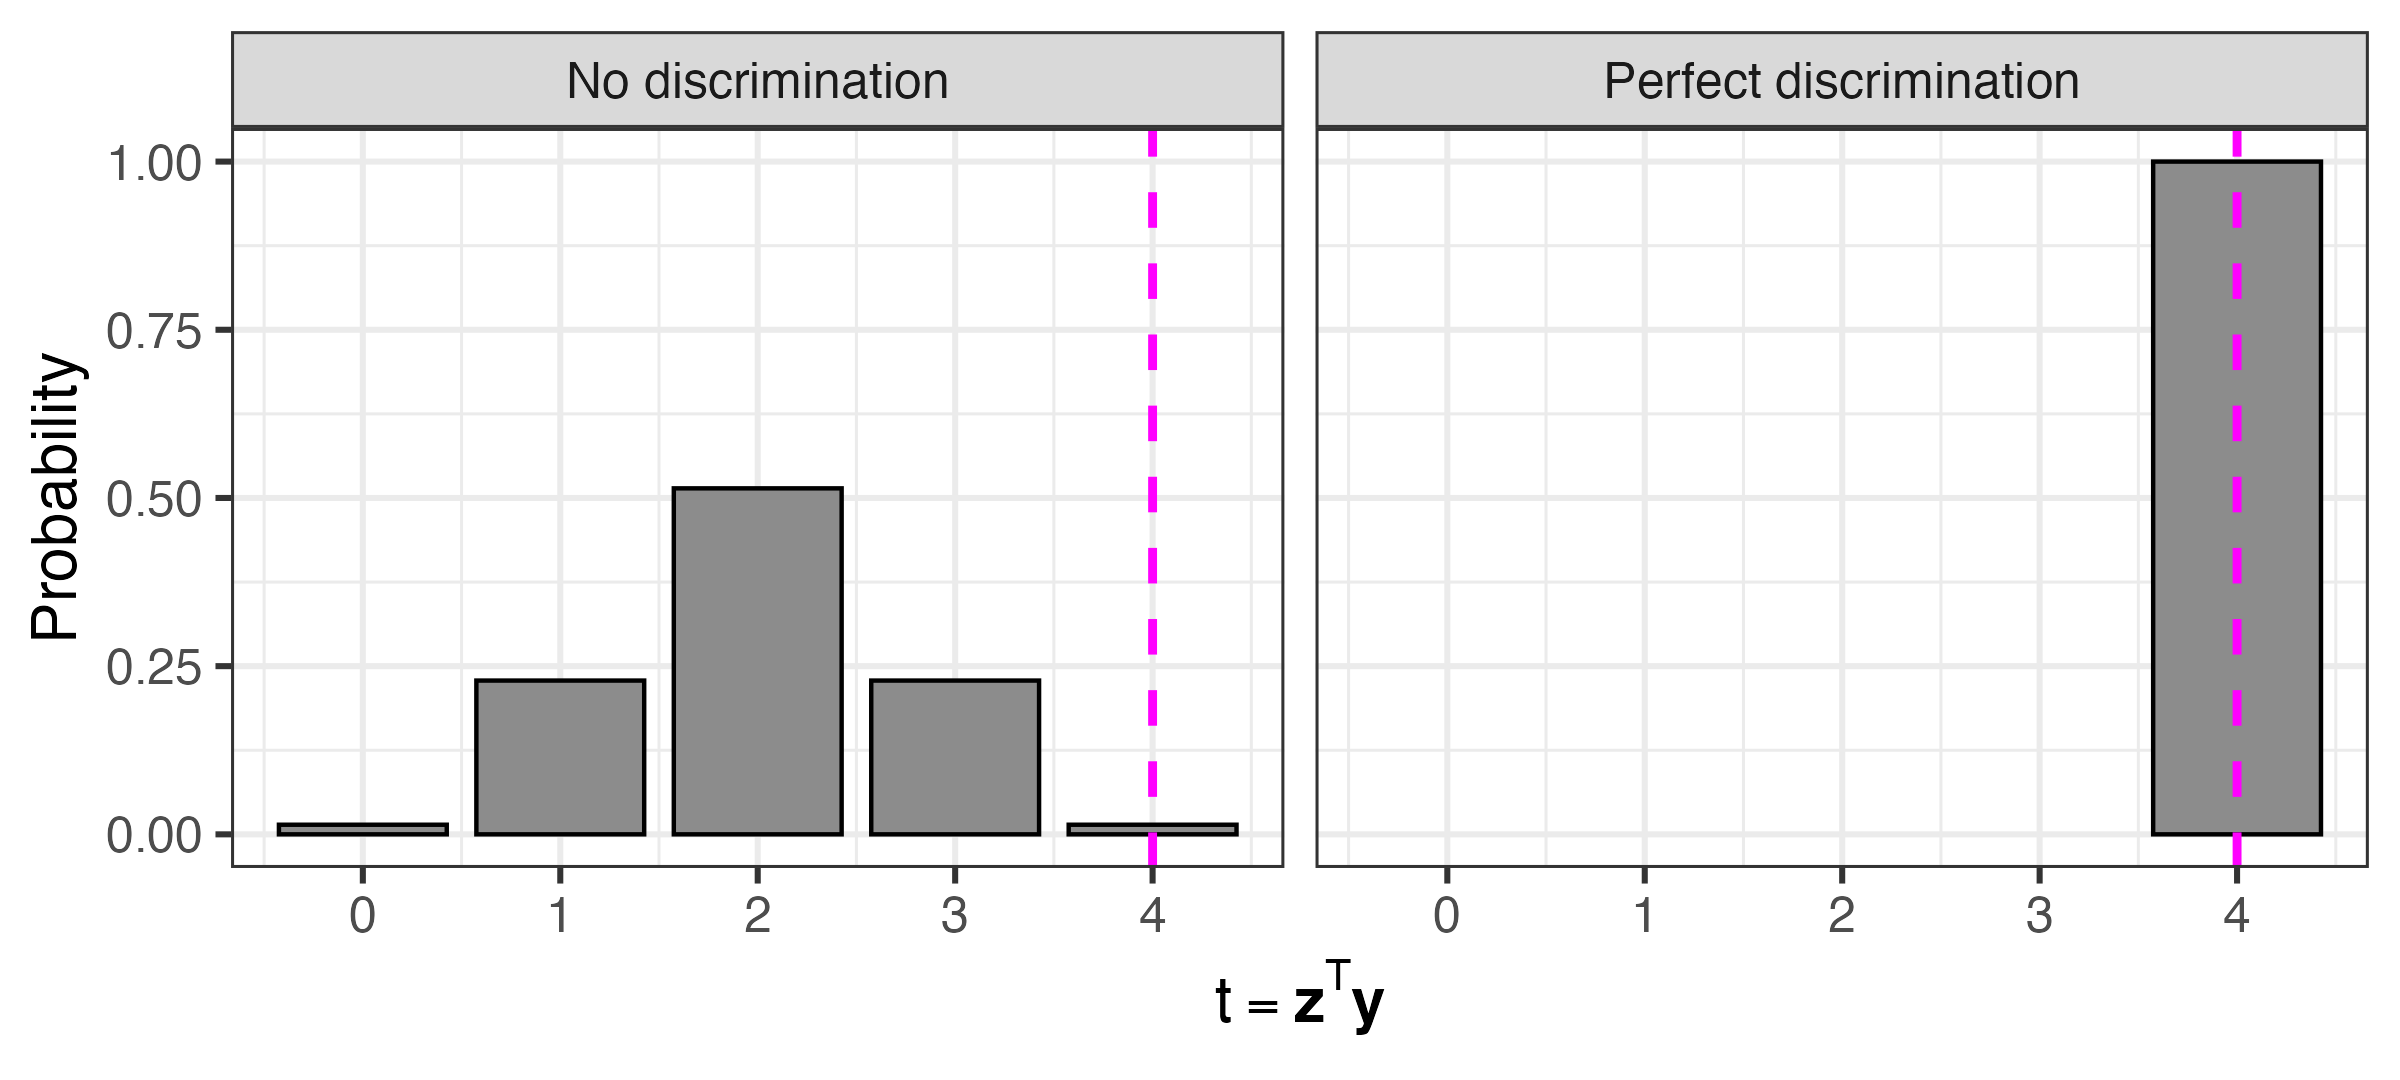
\includegraphics[width=0.92\linewidth,height=0.5\textheight,keepaspectratio]{figures/fisher_two_models.png}
\end{center}
\vfill
\begin{itemize} \vfill
\item Under no discrimination: Observed $4$ is extreme \vfill
\item Under perfect discrimination: Observed $4$ is ordinary \vfill
\item Same design, different model, different randomization distribution \vfill
\end{itemize} \vfill
\end{frame}
%---------------------------------------------------------------
\begin{frame}{The logic in three parts}
\vfill
\begin{itemize} \vfill
\item \mh{Design} \\ known assignment mechanism $p(\bm{z})$ over $\Omega$ \vfill
\item \mh{Model} \\ a sharp causal model of each cup's two responses \vfill
\item \mh{Test} \\ distribution of $t(\bm{Z},\bm{y})$ under the model \vfill
\item Fisher's exact test: this logic with \mh{no discrimination} \vfill
\item Inference rests on the \mh{design}, not a sampled population \vfill
\end{itemize} \vfill
\end{frame}
%% ============================================================
%% PART 6 --- RECAP
%% ============================================================
\section{Recap}

\begin{frame}{Recap: why we randomize}
\vfill
\begin{itemize} \vfill
\item Same \mh{rule}: reject no discrimination when she gets all four correct \vfill
\item Random assignment determines this rule's \mh{error probabilities}: \vfill
\begin{itemize} \vfill
\item reject no discrimination when it is \mh{true}: $\Pr = 1/70 \approx 0.014$ \vfill
\item reject no discrimination when \mh{perfect discrimination} holds: $\Pr = 1$ \vfill
\end{itemize} \vfill
\item Both probabilities come from the \mh{design}, not assumptions \vfill
\item Randomization makes uncertainty \mh{known} with controlled errors \vfill
\item That is the value of random assignment: a \mh{reasoned basis for inference} \vfill
\end{itemize} \vfill
\end{frame}
%---------------------------------------------------------------
\begin{frame}
\frametitle{References} 
\scriptsize
\bibliographystyle{chicago}
\bibliography{Master_Bibliography}   % name your BibTeX data base
\end{frame}
%---------------------------------------------------------------
\end{document}